\ifx\allfiles\undefined
\documentclass[12pt, a4paper, oneside, UTF8]{ctexbook}
\def\path{../config}
\usepackage{amsmath}
\usepackage{amsthm}
\usepackage{amssymb}
\usepackage{array}
\usepackage{xcolor}
\usepackage{graphicx}
\usepackage{mathrsfs}
\usepackage{enumitem}
\usepackage{geometry}
\usepackage[colorlinks, linkcolor=black]{hyperref}
\usepackage{stackengine}
\usepackage{yhmath}
\usepackage{extarrows}
\usepackage{tikz}
\usepackage{pgfplots}
\usepackage{asymptote}
\usepackage{float}
\usepackage{fontspec} % 使用字体

\setmainfont{Times New Roman}
\setCJKmainfont{LXGWWenKai-Light}[
    SlantedFont=*
]

\everymath{\displaystyle}

\usepgfplotslibrary{polar}
\usepackage{subcaption}
\usetikzlibrary{decorations.pathreplacing, positioning}

\usepgfplotslibrary{fillbetween}
\pgfplotsset{compat=1.18}
% \usepackage{unicode-math}
\usepackage{esint}
\usepackage[most]{tcolorbox}

\usepackage{fancyhdr}
\usepackage[dvipsnames, svgnames]{xcolor}
\usepackage{listings}

\definecolor{mygreen}{rgb}{0,0.6,0}
\definecolor{mygray}{rgb}{0.5,0.5,0.5}
\definecolor{mymauve}{rgb}{0.58,0,0.82}
\definecolor{NavyBlue}{RGB}{0,0,128}
\definecolor{Rhodamine}{RGB}{255,0,255}
\definecolor{PineGreen}{RGB}{0,128,0}

\graphicspath{ {figures/},{../figures/}, {config/}, {../config/} }

\linespread{1.6}

\geometry{
    top=25.4mm, 
    bottom=25.4mm, 
    left=20mm, 
    right=20mm, 
    headheight=2.17cm, 
    headsep=4mm, 
    footskip=12mm
}

\setenumerate[1]{itemsep=5pt,partopsep=0pt,parsep=\parskip,topsep=5pt}
\setitemize[1]{itemsep=5pt,partopsep=0pt,parsep=\parskip,topsep=5pt}
\setdescription{itemsep=5pt,partopsep=0pt,parsep=\parskip,topsep=5pt}

\lstset{
    language=Mathematica,
    basicstyle=\tt,
    breaklines=true,
    keywordstyle=\bfseries\color{NavyBlue}, 
    emphstyle=\bfseries\color{Rhodamine},
    commentstyle=\itshape\color{black!50!white}, 
    stringstyle=\bfseries\color{PineGreen!90!black},
    columns=flexible,
    numbers=left,
    numberstyle=\footnotesize,
    frame=tb,
    breakatwhitespace=false,
} 

\lstset{
    language=TeX, % 设置语言为 TeX
    basicstyle=\ttfamily, % 使用等宽字体
    breaklines=true, % 自动换行
    keywordstyle=\bfseries\color{NavyBlue}, % 关键字样式
    emphstyle=\bfseries\color{Rhodamine}, % 强调样式
    commentstyle=\itshape\color{black!50!white}, % 注释样式
    stringstyle=\bfseries\color{PineGreen!90!black}, % 字符串样式
    columns=flexible, % 列的灵活性
    numbers=left, % 行号在左侧
    numberstyle=\footnotesize, % 行号字体大小
    frame=tb, % 顶部和底部边框
    breakatwhitespace=false % 不在空白处断行
}

% \begin{lstlisting}[language=TeX] ... \end{lstlisting}

% 定理环境设置
\usepackage[strict]{changepage} 
\usepackage{framed}

\definecolor{greenshade}{rgb}{0.90,1,0.92}
\definecolor{redshade}{rgb}{1.00,0.88,0.88}
\definecolor{brownshade}{rgb}{0.99,0.95,0.9}
\definecolor{lilacshade}{rgb}{0.95,0.93,0.98}
\definecolor{orangeshade}{rgb}{1.00,0.88,0.82}
\definecolor{lightblueshade}{rgb}{0.8,0.92,1}
\definecolor{purple}{rgb}{0.81,0.85,1}

\theoremstyle{definition}
\newtheorem{myDefn}{\indent Definition}[section]
\newtheorem{myLemma}{\indent Lemma}[section]
\newtheorem{myThm}[myLemma]{\indent Theorem}
\newtheorem{myCorollary}[myLemma]{\indent Corollary}
\newtheorem{myCriterion}[myLemma]{\indent Criterion}
\newtheorem*{myRemark}{\indent Remark}
\newtheorem{myProposition}{\indent Proposition}[section]

\newenvironment{formal}[2][]{%
	\def\FrameCommand{%
		\hspace{1pt}%
		{\color{#1}\vrule width 2pt}%
		{\color{#2}\vrule width 4pt}%
		\colorbox{#2}%
	}%
	\MakeFramed{\advance\hsize-\width\FrameRestore}%
	\noindent\hspace{-4.55pt}%
	\begin{adjustwidth}{}{7pt}\vspace{2pt}\vspace{2pt}}{%
		\vspace{2pt}\end{adjustwidth}\endMakeFramed%
}

\newenvironment{definition}{\vspace{-\baselineskip * 2 / 3}%
	\begin{formal}[Green]{greenshade}\vspace{-\baselineskip * 4 / 5}\begin{myDefn}}
	{\end{myDefn}\end{formal}\vspace{-\baselineskip * 2 / 3}}

\newenvironment{theorem}{\vspace{-\baselineskip * 2 / 3}%
	\begin{formal}[LightSkyBlue]{lightblueshade}\vspace{-\baselineskip * 4 / 5}\begin{myThm}}%
	{\end{myThm}\end{formal}\vspace{-\baselineskip * 2 / 3}}

\newenvironment{lemma}{\vspace{-\baselineskip * 2 / 3}%
	\begin{formal}[Plum]{lilacshade}\vspace{-\baselineskip * 4 / 5}\begin{myLemma}}%
	{\end{myLemma}\end{formal}\vspace{-\baselineskip * 2 / 3}}

\newenvironment{corollary}{\vspace{-\baselineskip * 2 / 3}%
	\begin{formal}[BurlyWood]{brownshade}\vspace{-\baselineskip * 4 / 5}\begin{myCorollary}}%
	{\end{myCorollary}\end{formal}\vspace{-\baselineskip * 2 / 3}}

\newenvironment{criterion}{\vspace{-\baselineskip * 2 / 3}%
	\begin{formal}[DarkOrange]{orangeshade}\vspace{-\baselineskip * 4 / 5}\begin{myCriterion}}%
	{\end{myCriterion}\end{formal}\vspace{-\baselineskip * 2 / 3}}
	

\newenvironment{remark}{\vspace{-\baselineskip * 2 / 3}%
	\begin{formal}[LightCoral]{redshade}\vspace{-\baselineskip * 4 / 5}\begin{myRemark}}%
	{\end{myRemark}\end{formal}\vspace{-\baselineskip * 2 / 3}}

\newenvironment{proposition}{\vspace{-\baselineskip * 2 / 3}%
	\begin{formal}[RoyalPurple]{purple}\vspace{-\baselineskip * 4 / 5}\begin{myProposition}}%
	{\end{myProposition}\end{formal}\vspace{-\baselineskip * 2 / 3}}


\newtheorem{example}{\indent \color{SeaGreen}{Example}}[section]
\renewcommand{\proofname}{\indent\textbf{\textcolor{TealBlue}{Proof}}}
\NewEnviron{solution}{%
	\begin{proof}[\indent\textbf{\textcolor{TealBlue}{Solution}}]%
		\color{blue}% 设置内容为蓝色
		\BODY% 插入环境内容
		\color{black}% 恢复默认颜色(可选,避免影响后续文字)
	\end{proof}%
}

% 自定义命令的文件

\def\d{\mathrm{d}}
\def\R{\mathbb{R}}
%\newcommand{\bs}[1]{\boldsymbol{#1}}
%\newcommand{\ora}[1]{\overrightarrow{#1}}
\newcommand{\myspace}[1]{\par\vspace{#1\baselineskip}}
\newcommand{\xrowht}[2][0]{\addstackgap[.5\dimexpr#2\relax]{\vphantom{#1}}}
\newenvironment{mycases}[1][1]{\linespread{#1} \selectfont \begin{cases}}{\end{cases}}
\newenvironment{myvmatrix}[1][1]{\linespread{#1} \selectfont \begin{vmatrix}}{\end{vmatrix}}
\newcommand{\tabincell}[2]{\begin{tabular}{@{}#1@{}}#2\end{tabular}}
\newcommand{\pll}{\kern 0.56em/\kern -0.8em /\kern 0.56em}
\newcommand{\dive}[1][F]{\mathrm{div}\;\boldsymbol{#1}}
\newcommand{\rotn}[1][A]{\mathrm{rot}\;\boldsymbol{#1}}

\newif\ifshowanswers
\showanswerstrue % 注释掉这行就不显示答案

% 定义答案环境
\newcommand{\answer}[1]{%
    \ifshowanswers
        #1%
    \fi
}

% 修改参数改变封面样式,0 默认原始封面、内置其他1、2、3种封面样式
\def\myIndex{0}


\ifnum\myIndex>0
    \input{\path/cover_package_\myIndex} 
\fi

\def\myTitle{考研数学笔记}
\def\myAuthor{Weary Bird}
\def\myDateCover{\today}
\def\myDateForeword{\today}
\def\myForeword{相见欢·林花谢了春红}
\def\myForewordText{
    林花谢了春红,太匆匆。
    无奈朝来寒雨晚来风。
    胭脂泪,相留醉,几时重。
    自是人生长恨水长东。
}
\def\mySubheading{以姜晓千强化课讲义为底本}



\usepackage{listings} % 用于插入代码

% 定义代码高亮风格
\lstset{
    basicstyle=\ttfamily\small,        % 基本字体样式(等宽小字体)
    keywordstyle=\color{blue},         % 关键字颜色
    commentstyle=\color{green},        % 注释颜色
    stringstyle=\color{red},           % 字符串颜色
    numbers=right,
    breaklines=true,                   % 自动换行
    frame=single,                      % 代码框边框
    rulecolor=\color{black},           % 边框颜色
    captionpos=b,                      % 标题位置(底部)
    showspaces=false,                  % 不显示空格标记
    showstringspaces=false,            % 不显示字符串中的空格标记
    language=C                         % 设置语言为 C
}
\begin{document}
% \input{\path/cover_text_\myIndex.tex}

\newpage
\thispagestyle{empty}
\begin{center}
    \Huge\textbf{\myForeword}
\end{center}
\myForewordText
\begin{flushright}
    \begin{tabular}{c}
        \myDateForeword
    \end{tabular}
\end{flushright}

\newpage
\pagestyle{plain}
\setcounter{page}{1}
\pagenumbering{Roman}
\tableofcontents

\newpage
\pagenumbering{arabic}
% \setcounter{chapter}{-1}
\setcounter{page}{1}

\pagestyle{fancy}
\fancyfoot[C]{\thepage}
\renewcommand{\headrulewidth}{0.4pt}
\renewcommand{\footrulewidth}{0pt}








\else
\fi

\chapter{计算机基础}
\begin{tcolorbox}
    \bt[1] 表示真题, \bl[1] 表示重点题 
\end{tcolorbox}
\section{数据结构}
\begin{enumerate}
    \item  评估下面这段代码的时间复杂度()
\begin{lstlisting}[language=C]
    int func(int n) {
        int i = 0, sum = 0;
        while(sum < n) sum += ++i;
        return i;
    }
\end{lstlisting}

    \item 评估下面这段代码的时间复杂度()
\begin{lstlisting}[language=C]
    int sum = 0;
        for(int i = 1; i < n; i *= 2)
            for (int j = 0; j < i; j++)
                sum++;
\end{lstlisting}

    \item 一个栈的入栈序列为\underline{$1,2,3,\ldots,n$},出栈序列是\underline{$P_1,P_2,P_3,\ldots,P_n$}.若
    $P_2=3$,则$P_3$的可能取值的个数可能是() \\
    A.n-1\qquad B.n-2\qquad C.n-3\qquad D.无法确认 

    \item 已知\underline{循环队列}存储在一维数组$A[0,\ldots,n-1]$中,且队列非空的时候front和rear分别指向队头和队尾.若初始时
    队列为空,且要求第一个进入队列的元素存储在$A[0]$,则初始时front和rear的值分别为() \\
    A.0,0\qquad\qquad B.0,n-1\qquad\qquad C.n-1,0\qquad\qquad D.n-1,n-1

    \item \underline{循环队列}放在一维数组$A[0,\ldots,M-1]$中,end1指向队头元素,end2指向队尾元素的后一个位置.
    假设队列两端都可以进行入队和出队操作,队列中最多能容纳$M-1$个元素.初始队列不为空.下列判断对空和队满的条件中,正确的是() \\
    A. 对空:end1\ ==\ end2; \qquad\qquad\qquad\qquad\quad 队满:end1\ ==\ (end2+1)mod\ M\\
    B. 对空:end1\ ==\ end2; \qquad\qquad\qquad\qquad\quad 队满:end2\ ==\ (end1+1)mod\ M-1\\
    C. 对空:end2\ ==\ (end1+1)mod\ M; \qquad\qquad 队满:end1\ ==\ (end2+1)mod\ M\\
    D. 对空:end1\ ==\ (end2+1)mod\ M; \qquad\qquad 队满:end2\ ==\ (end1+1)mod\ (M-1)
    
    \item \underline{火车重排问题}\\
    假设火车入口和出口之间有n条轨道,列车驶入的顺序为\underline{$8,4,2,5,3,9,1,6,7$}若希望
    得到的驶出顺序为 \underline{$1\sim 9$}则n至少为()\\
    A.2\qquad\qquad B.3\qquad\qquad C.4\qquad\qquad D.5

    \item 在一颗度为4的树T中,若有20个度为4的结点,10个度为3的结点,1个度为2的结点,10个度为1的结点,则树T
    的叶结点个数为() \\
    A.41\qquad\qquad B.82\qquad\qquad C.113\qquad\qquad D.122

    \item 已知一颗完全二叉树的第六层(设根为第一层)由8个叶结点,则该完全二叉树的结点个数\underline{最多为}() \\
    A.39\qquad\qquad B.52\qquad\qquad C.111\qquad\qquad D.119
    
    \item 若一颗完全二叉树有786个结点,则该二叉树中叶结点的个数为() \\
    A.257\qquad\qquad B.258\qquad\qquad C.384\qquad\qquad D.385

    \item 先序序列为\underline{$a,b,c,d$}的不同二叉树的个数为() \\
    A.13 \qquad\qquad B.14 \qquad\qquad C.15\qquad\qquad D.16

    \item 将森林转换为对应的二叉树,若在二叉树中,结点u是结点v的父结点的父结点,则在原来的森林中,u和v可能的关系是()
    \begin{enumerate}
        \item [(I)] 父子关系
        \item [(II)] 兄弟关系
        \item [(III)] u的父结点与v的父结点是兄弟关系
    \end{enumerate}

    \item 已知一颗有2011个结点的树,其叶结点的个数为116,该树对应的二叉树中\underline{无右孩子}的结点个数为()
    
    \item 已知森林F及与之对应的二叉树T,若F的先根遍历序列为\underline{$a,b,c,d,e,f$},中根遍历序列为\underline{$b,a,d,f,e,c$},则T的后根
    遍历序列为()

    \item 对任意给定的含n(n>2)个字符的有限集合S,用二叉树表示S的哈夫曼编码集与定长编码集,分别得到二叉树
    $T_1,T_2$.下列叙述中,正确的是() \\
    A. $T_1$和$T_2$的结点个数相同 \\
    B. $T_1$的高度大于$T_2$的高度 \\
    C. 出现频次不同的字符在$T_1$中处于不同的层 \\
    D. 出现频次不同的字符在$T_2$中处于相同的层

    \item 在由6个字符构成的字符集S中,各字符出现的频次为\underline{$3,4,5,6,8,10$},为S构造的哈夫曼树的
    加权平均长度为() \\
    A.2.4\qquad\qquad B.2.5\qquad\qquad C.2.67\qquad\qquad D.2.75

    \item 对于任意一棵高度为5且有10个结点的二叉树,若采用顺序存储结构保存,每个结点占一个存储单元,则存放该二叉树
    至少需要多少存储单元? 

    \item 在下列关于二叉树遍历的说法中, 正确的是 (   ).
    \begin{enumerate}
        \item[(A)]若有一个结点是二叉树中某个子树的中序遍历结果序列的最后一个结点, 则它一定
        是该子树的前序遍历结果序列的最后一个结点
        \item[(B)] 若有一个结点是二叉树中某个子树的前序遍历结果序列的最后一个结点, 则它一定
        是该子树的中序遍历结果序列的最后一个结点
        \item[(C)]若有一个叶结点是二叉树中某个子树的中序遍历结果序列的最后一个结点, 则它一
        定是该子树的前序遍历结果序列的最后一个结点
        \item[(D)] 若有一个叶结点是二叉树中某个子树的前序遍历结果序列的最后一个结点, 则它一
        定是该子树的中序遍历结果序列的最后一个结点
    \end{enumerate}

\end{enumerate}

\newpage
\section{计算机网络}

\begin{enumerate}
    \item 计算机网络可以被理解为() \\
    A. 执行计算机数据处理的软件模块 \\
    B. 由自治的计算机互联起来的集合体 \\
    C. 多个处理器通过共享内存视线的耦合系统 \\
    D. 用于共同完成一项任务的分布式系统 
    \answer{
        \begin{solution}
        选B \\
        计算机网络是由\underline{自治计算机互连起来的集合体.} 其中包含三个关键点:自治计算机,互连,集合体.
        其中自治计算机有\underline{硬件和软件}两部分组成,能完成地实现计算机的各种功能;互连是指计算机之间能实现
        \underline{相互通信}.
        \end{solution}
    }
    \item 下列不属于计算机网络功能的是() \\
    A. 提高系统的可靠性\qquad B.提高工作效率 \\
    C. 分散数据的综合处理 \qquad D. 使各计算机相对独立 
    
    \answer{
        \begin{solution}
            选D \\
            计算机网络的功能为\underline{数据通信,资源共享以及分布式处理}
        \end{solution}
    }

    \item 在计算机中可以没有的是() \\
    A. 客户机 \qquad B. 服务器\qquad C.操作系统\qquad D.数据库管理系统 

    \answer{
        \begin{solution}
            选D \\
            从物理组成上看,计算机网络由硬件、软件和协议组成.客户机是客户访问网络的出入口,服务器是提供服务、存储信息的设备
        \end{solution}
    }

    \item 局域网和广域网的差异不仅在于它们所覆盖的范围不同,还主要在于它们() \\
    A.所使用的介质不同\qquad B.所使用的协议不同 \\
    C.所能支持的通信量不同\qquad D.所提供的服务不同

    \answer{
        \begin{solution}
            选B \\
            局域网使用广播技术(CSMA/CD或者CSMA/CA为主要协议)而广域网普遍使用点对点技术(P2P协议为主要协议)
        \end{solution}
    }

    \item 广域网的拓扑结构通常为() \\
    A.星型\qquad B.总线型\qquad C.网状\qquad D.环形

    \answer{
        \begin{solution}
            选C
        \end{solution}
    }


    \item \bl OSI参考模型中数据链路层不具有的功能是() \\
    A.物理寻址\qquad B.流量控制\qquad C.差错检验\qquad D.拥塞控制

    \answer{
        \begin{solution}
            选D \\
            数据链路层在\underline{不可靠的物理层}上提供可靠的传输,其主要功能为\textbf{成帧,物理寻址,流量控制
            ,差错检验,数据重发}等,拥塞控制是网络层与传输层的概念.
        \end{solution}
    }

    \item \bl 在ISO/OSI参考模型中,可同时提供无连接服务和面向连接服务的是() \\
    A.物理层\qquad B.数据链路层\qquad C.网络层\qquad D.传输层
    
    \answer{
        \begin{solution}
            选C \\
            这道题考察TCP/IP协议栈和ISO/OSI参考模型的区别. ISO/OSI在网络层提供无连接服务和面向连接服务;
            但在传输层仅支持面向连接到通信;TCP/IP协议栈,网络层仅支持无连接服务;而传输层提供无连接服务和面向连接服务
        \end{solution}
    }
    \item \bl[1] 二进制信号在信噪比为127:1的4kHz的信道上传输,最大数据传输速率可达到() \\
    A.28000bps\qquad B.8000bps\qquad C.4000bps\qquad D.无限大

    \answer{
        \begin{solution}
            考虑奈氏定理有
            $$
            R_{max} = 2 \times 4k \times \log_{2}{2} = 8 kbps 
            $$
            考虑香农定理有 
            $$
            R_{max} = 4k \times \log_{2}(1+127) = 28 kbps
            $$
            最大带宽(数据传输速率)受限于二者的较小值,即$R_{max} = 8kbps$
        \end{solution}
    }
    \item 为了使数据在网络中的传输延迟最小,首选的交换方式是() \\
    A.电路交换\qquad B.报文交换\qquad C.分组交换\qquad D.信元交换 
    
    \answer{
        \begin{solution}
            答案选A,电路交换的特点就是实时性好.
        \end{solution}
        \begin{tcolorbox}[title=四种交换方式的一图流]
            \begin{tabular}{|c|c|c|}
                \hline 
                交换方式&特点(优点)&缺点 \\
                \hline
                电路交换&\begin{tabular}{c}
                    独占信道 \\
                    实时性强,无冲突 \\
                    数据顺序到达 
                \end{tabular} & \begin{tabular}{c}
                    建立时间长 \\
                    信道利用率低 \\
                    灵活性差 \\
                    不具备差错控制能力 
                \end{tabular} \\
                \hline
                报文交换 & \begin{tabular}{c}
                    不需要预先建立连接 \\
                    动态分配链路资源 \\
                    支持多目标广播 \\
                    不划分报文 
                \end{tabular} &\begin{tabular}{c}
                    存储转发延迟高 \\
                    需要较大的存储空间 \\
                    不适合实时通信
                \end{tabular} \\
                \hline 
                虚电路分组交换​ & \begin{tabular}{c}
                    分组按序到达 \\
                    资源动态共享 \\
                    差错控制由网络层负责
                \end{tabular} & \begin{tabular}{c}
                    需要需要建立连接 \\
                    路由故障需要重新建立 \\
                    有额外的开销
                \end{tabular} \\ 
                \hline
                数据分组交换 & \begin{tabular}{c}
                    无须连接建立,灵活高效 \\
                    健壮性强 \\
                    适合短报文,突发流量
                \end{tabular} & \begin{tabular}{c}
                    分组可能失序,丢失 \\
                    网络部保证可靠性 \\
                    每个分组需要携带完整的地址 
                \end{tabular} \\
                \hline
            \end{tabular}
        \end{tcolorbox} 
    }

    \item 下列关于三种数据交换方式的叙述,错误的是() \\
    A.电路交换不提供差错控制功能 \\
    B.分组交换的分组有最大长度限制 \\
    C.虚电路是面向连接的,它提供的是一种可靠服务 \\
    D.在出错率很高的传输系统中,选择虚电路方式更合适 

    \answer{
        \begin{solution}
            选D,简单立即的话就是虚电路所有分组按照同一虚电路传输,出错率较高容易出现结点故障;此时就
            需要重新建立虚电路耗费极大.而数据报可以任意路由,部分结点即使故障也不影响.
        \end{solution}
    }
    \item 同一报文中的分组可以由不同的传输路径通过通信子网的方法是()  \\
    A.分组交换\qquad B.电路交换\qquad C.虚电路\qquad D.数据报

    \answer{
        \begin{solution}
            选D
        \end{solution}
    }
    \item 下列4中传输方法中,由网络负责差错控制和流量控制,分组按顺序被递交的是() \\
    A.电路交换\qquad B.报文交换\qquad C.虚电路分组交换 \qquad D.数据报分组交换 

    \answer{
        \bs{
            选C 
        }
    }

    \item 利用一根同轴电缆互联主机构成以太网,则主机间的通信方式为() \\
    A.全双工\qquad B.半双工\qquad C.单工\qquad D.不能确定
    
    \answer{
        \bs{
            这道题吧,其实没啥道理.单纯想总结一下传统以太网(10BASE-T)的特点. 
            \begin{enumerate}
                \item [(1)] 采用CSMA/CD协议 
                \item [(2)] 共享总线型拓扑结构,通过集线器连接;所有主机共享带宽
                \item [(3)] 最小帧长$64B$,数据范围$46B\sim 1500B$
                \item [(4)] 半双工通信
                \item [(5)] 采用曼彻斯特编码
            \end{enumerate}
            对比一下现代交换式以太网(高速以太网 $100Mbps,1Gbps,10Gbps$) 
            \begin{enumerate}
                \item [(1)] 拓扑结构通常为星型(交换机为主要设备) 
                \item [(2)] 独享带宽(交换机的特性)
                \item [(3)] 全双工通信
                \item [(4)] 每个端口是一个冲突域(交换机的特性)
                \item [(5)] 弃用曼彻斯特编码
            \end{enumerate}
        }
    }

    \item 两个网段在物理层进行互联时要求() \\
    A.数据传输速率和数据链路层协议都可以不同 \\
    B.数据传输速率和数据链路层协议都要相同 \\
    C.数据传输速率要相同,但数据链路层协议可以不同 \\
    D.数据传输速率可以不同,但数据链路层要相同

    \answer{
        \bs {
            选C,由于数据传输速率不同会导致数据丢失或者效率低下(没有流量控制),而数据链路层协议在物理层上层
            与物理层互连无关; 若是要求数据链路层互连,则协议也要相同.
        }
    }
    \item \bl[2] 要发送的数据是\underline{1101\ 0110\ 11},采用CRC校验,生成多项式是10011,那么最终发送的
    数据应该是() \\
    A.\underline{1101\ 0110\ 1110\ 10} \qquad B.\underline{1101\ 0110\ 1101\ 10}  \\
    C.\underline{1101\ 0110\ 1111\ 10} \qquad C.\underline{1111\ 0011\ 0111\ 00}
    
    \answer{
        \bs{
            答案为 C
        }

        \begin{remark}[CRC的计算方法]
            \begin{enumerate}
                \item [(1)] 根据给的生成多项式$G(x)$其的阶数$n$,往要发送的数据后加入$n$个零
                \item [(2)] 将上面得到的01串与生成多项式做模2除法(加减法做异或操作) 
                \item [(3)] 得到的\textbf{余数}加入原发送数据,并发送给接收方
                \item [(4)] 接收方接收到数据后,与生成多项式做模2除法,若余数为0则无差错否则出错  
            \end{enumerate}
        \end{remark}
    }

    \item 数据链路层采用后退N帧协议方式,进行流量控制和差错控制,发送方已经发送了编号$0\sim 6$的帧,计时器超时时,
    仅收到了对$1,3,5$好帧的确认,发送方需要重传的帧数目是() \\
    A. 1\qquad B.2 \qquad C.5\qquad D.6

    \answer{
        \bs {
            选A, 显然采用了累积确认,最后收到的确认是$5$说明$0\sim 5$号帧以被接受,只有$6$需要重传
        }
    }
    \item 一个使用选择重传协议的数据链路层协议,如果采用5位的帧序列号,那么可以选择的最大接受窗口是() \\
    A.15\qquad B.16\qquad C.31\qquad D.32

    \answer{
        \bs {
            选B \\
            这道题比较有争议,有的书上说最大接受窗口要满足$W_{R}\leq 2^{n-1},W_{R}=W_{A}$而有的只要
            满足$W_{R}\leq 2^n - 1,W_{A}=1$ 即可,王道这里采用的是前者的说法. 
        }
    }
    \item 对于窗口大小为$n$的滑动窗口,最多可以有()帧以发送但还没有确认 \\
    A. 0 \qquad B.n-1\qquad C.n\qquad D.n/2 

    \answer{
        \bs {
            选B \\
            滑动窗口协议中,发送方窗口的大小$W_{A}\leq n - 1$,故同一时间至多有$n-1$个帧以发送而未被确认. 
        }
    }

    \item \bt[1] 主机甲采用停止等待协议向主机乙发送数据,数据传输速率是$3kb/s$,单向传播时延是$200ms$忽略
    确认帧的延迟.当信道利用率达到$40\%$时,数据帧的长度是() \\
    A.240比特\qquad B.400比特\qquad C.480比特\qquad D.800比特
    
    \answer{
        \bs {

        }
    }
    \item 从表面看,$FDM$比$TDM$能更好地利用信道的传输能力,但现在计算机网络更多地使用TDM而非FDM的原因是() \\
    A.FDM实际能力更差\qquad B.TDM可以用于数字传输而FDM不行 \\
    C.FDM技术更成熟\qquad D.TDM能更充分利用带宽

    \item 长度为$10km$数据传输速率为$10Mb/s$的CSMA/CD以太网,信号传播速率为$200m/\mu s$那么该网络的最小
    帧长为() \\
    A.$20bit$ \qquad B.$200bit$\qquad C.$100bit$\qquad D.$1000bit$
    
    \item 与$CSMA/CD$网络相比,令牌环网更适合的环境是() \\
    A.负载轻\qquad B.负载重\qquad C.距离远\qquad D.距离近

    \item 无线局域网不使用$CSMA/CD$而使用$CSMA/CA$的原因是,无线局域网() \\
    A.不能同时收发,无法在发送时接受信号 \\
    B.不需要再发送过程中进行冲突检测 \\
    C.无线信号的广播特性,使得不会出现冲突 \\
    D.覆盖范围小,不进行冲突检测不能影响正确性 

    \item 多路复用器的主要功能是() \\
    A.执行模/数转换\qquad B.执行串行/并行转换 \\
    C.减少主机的通信处理负荷\qquad D.结合来自两条或更多线路的传输 

    \item 下列关于令牌环网的说法中,不正确的是() \\
    A.媒体的利用率比较公平 \\
    B.重负载下信道利用率高 \\
    C.结点可以一直持有令牌,直到所要发送的数据传输完毕 \\
    D.令牌是一种特殊的控制帧 
    
    \item \bt 下列选中,对正确接受到的数据帧进行确认的协议是()\\
    A.CSMA\qquad B.CDMA\qquad C.CSMA/CD\qquad CSMA/CA 

    \item \bt 下列介质访问控制方法中,可能发生冲突的是() \\
    A.CDMA\qquad B.CSMA\qquad C.TDMA\qquad D.FDMA

    \item 以下关于以太网的说法中,正确的是() \\
    A.以太网的物理拓扑结构是总线型 \\
    B.以太网提供有确认的无连接服务 \\
    C.以太网参考模型一般只包括物理层和数据链路层 \\
    D.以太网必须使用CSMA/CD协议

    \item 在以太网中,大量的广播信息会降低整个网络性能的原因是() \\
    A.网络中的每台计算机都必须为每个广播信息发送一个确认信息 \\
    B.网络中的每台计算机都必须处理每个广播信息 \\
    C.广播信息被路由器自动路由到每个网段 \\
    D.广播信息不能直接自动的传送到目的计算机 

    \item 在一个以太网中,由$A,B,C,D$四台主机,若$A$向$B$发送数据,则() \\
    A.只有$B$可以接受到数据\qquad B.四台主机都能接受到数据 \\
    C.只有$B,C,D$可以接受到数据\qquad D.四台主机都不可以接受到数据 

    \item 下列关于吉比特以太网的说法中,错误的是() \\
    A.支持流量控制机制 \\
    B.采用曼彻斯特编码,利用光纤进行数据传输 \\
    C.数据的传输时间主要受线路传输延迟的限制 \\
    D.同时支持全双工模式和半双工模式 
    
    \item 下列关于虚拟局域网(VLAN)的说法中,错误的是() \\
    A.虚拟局域网建立在交换技术至上 \\
    B.虚拟局域网通过硬件方式实现逻辑分组和管理\\
    C.虚拟网的划分和计算机的实际物理位置无关 \\
    D.虚拟局域网中的计算机可以处于不同的局域网中
    
    \item 下列关于广域网和局域网的描述中,正确的是() \\
    A.广域网和互联网相似,可以连接不同类型的网络 \\
    B.在$OSI$参考模型层次结构中,广域网和局域网均涉及物理层,数据链路层和网络层 \\
    C.从互联网的角度看,广域网和局域网是平等的 \\
    D.局域网即以太网,其逻辑结构是总线结构 

    \item 若一个网络采用一个具有24个$10Mb/s$端口的半双工交换机作为连接设备,则每个连接点平均获得的带宽为
    ()该交换机的总容量为()

    \item \bt 对于$10Mb/s$的以太网交换机,当输出端口无排队,以直通交换的方式转发一个以太网帧(不包括前导码)
    引入的转发时延至少是() \\
    A.$0\mu s$\qquad B.$0.48\mu s$\qquad C.$5.12\mu s$\qquad D.$121.44\mu s$ 


    \item 网络层的主要目的是() \\
    A.在临接结点间进行数据报传输\qquad B.在临接结点间进行数据报的可靠传输 \\
    C.在任意结点间进行数据报传输\qquad C.在任意结点间进行数据报的可靠传输

    \item 路由器连接的异构网络是指() \\
    A.网络的拓扑结构不同\qquad B.网络中的计算机操作系统不同\\
    B.数据链路层和物理层均不同\qquad D.数据链路层协议相同,物理层协议不同 

    \item 在距离-向量路由协议中,()最可能导致路由回路的问题. \\
    A.由于网络带宽的限制,某些路由更新数据报被丢弃 \\
    B.由于路由器不知道整个网络的拓扑结构信息,当收到一个路由更新消息时,又将该更新消息发回自己发送该路由信息的路由器 \\
    C.当一个路由器发现自己的一条直接相邻链路断开时,未能将这个变化报告给其他路由器\\
    D.慢收敛导致路由器接受了无效的路由信息

    \item 以下关于IP分组分片基本方法的描述中,错误的是() \\
    A. IP分组长度大于MTU时,就必须对其进行分片 \\
    B. DF=1,分组长度又超过MTU时,则丢弃该分组,不需要向源主机报告 \\
    C.分片的MF值为1表示接受到的分片不是最后一个分片 \\
    D.属于同一原始IP分组的分片具有相同的标识

    \item 路由器R0的路由表见下,若进入路由器R0的分组的目标地址为\underline{132.19.237.5},则该分组应该被转发到()下
    一跳路由器.
    $$
    \begin{tabular}{lc} % @{} 去除首尾多余空白
    \toprule
    \text{目的网络} & \text{下一条} \\
    \midrule
    \underline{132.0.0.0/8}   & R1   \\
    \underline{132.19.0.0/11}   & R2  \\
    \underline{132.19.232.0/22} & R3 \\
    \underline{0.0.0.0/0} & R4 \\
    \bottomrule
    \end{tabular}
    $$
    A. R1\qquad B.R2\qquad C.R3\qquad D.R4 

    \item 下列地址中属于单播地址的是() \\
    A.\underline{172.31.128.255/18}\qquad B.\underline{10.255.255.255}\qquad
    C.\underline{192.168.24.59/30}\qquad D.\underline{224.105.5.211}

    \item 访问因特网的每台主机都需要分配IP地址(假设采用默认子网掩码),下列可以分配给主机的IP地址是() \\
    A.\underline{192.46.10.0}\qquad B.\underline{110.47.10.0}\qquad
    C.\underline{127.10.10.17}\qquad D.\underline{211.60.256.21}

    \item 一个网段的网络号为\underline{198.0.10.0/27}则最多可以分成()个子网,每个子网最多具有()个有效的IP地址 \\
    A.8,\ 30\qquad B.4,\ 62\qquad C.16,\ 14\qquad D.32,\ 6 

    \item 一个网络中有几个子网,其中一个已分配了子网号\underline{74.178.247.96/29},则下列网络前缀中不能再
    分配给其他子网的是() \\
    A.\underline{74.178.247.120/29}\quad B.\underline{74.178.247.64/29}\quad
    C.\underline{74.178.247.96/28}\quad D.\underline{74.178.247.104/29}

    \item 主机A和主机B的IP地址分别为\underline{216.12.31.20}何\underline{216.13.32.21},要想让A和B工作在
    同一个IP子网内,应该给它们分配的子网掩码是() \\
    A.\underline{255.255.255.0}\qquad B.\underline{255.255.0.0}\qquad C.\underline{255.255.255.255}\qquad D.\underline{255.0.0.0}

    \item 某单位分配了一个B类地址,计划将内部网络划分为35个子网,将来可能增加16个子网,每个子网的主机数目将近800台
    ,则可行的掩码方案是() \\
    A.\underline{255.255.248.0}\qquad B.\underline{255.255.252.0}\qquad C.\underline{255.255.254.0}\qquad D.\underline{255.255.255.0}

    \item 下列IP地址中,只能作为IP地址的源IP地址但不能作为目的IP地址的是() \\
    A.\underline{0.0.0.0}\qquad B.\underline{127.0.0.1}\qquad C.\underline{200.10.10.3}\qquad D.\underline{255.255.255.255}

    \item 若将\underline{101.200.16.0/20}划分为5个子网,则可能的最小子网的可分配IP地址数是() \\
    A.126\qquad B.254\qquad C.510\qquad D.1022

    \item 现将一个IP网络划分为3个子网,若其中一个子网是\underline{192.168.9.128/26},则下列网络中,不可能是另外两个子网之一的是() \\
    A.\underline{192.168.9.0/25}\quad B.\underline{192.168.9.0/26}\quad C.\underline{192.168.9.192/26}\quad D.\underline{192.168.9.192/27}

    \item 若某主机的IP地址是\underline{183.80.72.48},子网掩码是\underline{255.255.192.0}则该主机所在网络的网络地址是() \\
    A.\underline{183.80.0.0}\qquad B.\underline{183.80.64.0}\qquad C.\underline{183.80.72.0}\qquad D.\underline{183.80.192.0}

    \item BGP交换的网络可达性信息是() \\
    A.到达某个网络所经过的路径\qquad B.到达某个网络的下一跳路由器 \\
    C.到达某个网络的链路状态摘要信息\quad D.到达某个网络的最短距离及其下一跳路由器

    \item 以下关于IP组播的概念描述中,错误的是() \\
    A.在单播路由选择中,路由器只能从它的一个接口转发收到的分组 \\
    B.在组播路由选择中,路由器可以从它的多个接口转收到的分组 \\
    C.用多个单播仿真一个组播时需要更多的带宽 \\
    D.在用多个单播仿真一个组播时,时延基本是相同的

    \item 在设计组播路由时,为了避免路由环路,() \\
    A.采用了水平分割技术\qquad B.构建组播转发树\\ 
    C.采用了IGMP\qquad D.通过生存时间(TTL)字段 

    \item 关于路由器的下列说法中,正确的是() \\
    A.路由器处理的信息量比交换机少,因此转发速度比交换机快 \\
    B.对于同一目标,路由器只提供延迟最小的最近路由 \\
    C.通常的路由器可以支持多种网络层协议,并提供不同协议之间的分组转发 \\
    D. 路由器不但能根据IP地址进行转发,而且可以根据物理地址进行转发

    \item 下列网络设备中,传输延迟时间最大的是() \\
    A.局域网交换机\qquad B.网桥\qquad C.路由器\qquad D.集线器 

    \item 在采用TCP连接的数据传输阶段,如果发送端的发送窗口值有1000变成2000,那么发送端在收到一个
    确认前可以发送() \\
    A.2000个TCP报文段 \qquad B.2000B \qquad C.1000B\qquad D.1000个TCP报文段

    \item TCP中滑动窗口的值设置太大,对主机的影响是() \\
    A.由于传送的数据过多而使路由器变得拥挤,主机可能丢失分组 \\
    B.产生过多ACK \\
    C.由于接受的数据多,而使主机的工作速度加快 \\
    D.由于接受的数据多,而使主机的工作速度变慢 

    \item 以下关于TCP窗口与拥塞控制概念的描述中,错误的是() \\
    A.接受端窗口(rwnd)通过TCP首部中的窗口字段通知数据的发送方 \\
    B.发送窗口的依据是 : 发送窗口 $\min{\left[\text{接收端窗口},\text{拥塞窗口}\right]}$ \\
    C.拥塞窗口是接收端根据网络拥塞情况确定的窗口值 \\
    D.拥塞窗口大小在开始时可以按指数规律增长

    \item 设TCP的拥塞窗口的慢开始门限值初始为8(单位为报文段),当拥塞窗口上升到12时发生超时,TCP开始慢启动
    和拥塞避免,那么第13次传输时候的拥塞窗口大小为() \\
    A.4\qquad B.6\qquad C.7\qquad D.8

    \item 主机甲和主机乙之间建立一个TCP连接,主机甲向主机乙发送了两个连续的TCP报文段,分别包含300B和500B的有效载荷,第一个
    段的序列号为200,主机乙正确接受到两个数据段后,发送给主机甲的确认序号是() \\
    A.500\qquad B.700\qquad C.800\qquad D.1000

    \item 若甲向乙发送一个TCP连接,最大段长MSS=1KB,RTT=5ms,乙开辟的接受缓存为64KB,则甲从建立成功至
    发送窗口达到32KB,需要经过的时间至少是() \\
    A.25ms\qquad B.30ms\qquad C.160ms\qquad D.165ms

    \item 若用户首先向服务器发送FIN段请求断开TCP连接,则当客户收到服务器发送的FIN段并向服务器发送ACK段后,客户的TCP
    状态转换为() \\
    A.CLOSE\_WAIT \qquad B.TIME\_WAIT\qquad C.FIN\_WAIT\_1\qquad D.FIN\_WAIT\_2

    \item 下列关于用户/服务器模型的说法中,不正确的是() \\
    A.服务器专用于完成某些服务,而客户机则作为这些服务的使用者 \\
    B.客户机通常位于前端,服务器通常位于后端 \\
    C.客户机和服务器通过网络实现协同计算任务 \\
    D.客户机是面向任务的,服务器是面向用户的

    \item 域名与()具有一一定义的关系 \\
    A.IP地址\qquad B.MAC地址\qquad C.主机\qquad D.以上都不是

    \item 域名系统(DNS)的组成中不包括() \\
    A.域名空间\qquad B.分布式数据库 \\
    C.域名服务器\qquad D.从内部IP地址到外部IP地址的翻译程序

    \item ()可以将其管辖的主机名转换为主机的IP地址 \\
    A.本地域名服务器\qquad B.根域名服务器 \\
    C.授权域名服务器\qquad D.代理域名服务器 

    \item 若本地域名服务器无缓存,则在采用递归方法解析另一网络某主机域名时,用户主机和本地域名服务器发送的域名请求条数分别为() \\
    A.1条,\ 1条\qquad B.1条,\ 多条\qquad C.多条,\ 1条\qquad D.多条,\ 多条

    \item 假设所有域名服务器采用迭代查询进行域名解析,当主机访问规范域名\underline{www.abc.xyz.cn}的网站时,
    本地域名服务器在完成该域名解析的过程中,可能发出的DNS查询的最少和最多次数分别是() \\
    A.0,\ 3\qquad B.1,\ 3\qquad C.0,\ 4\qquad D.1, 4

    \item 假设下列网络中的本地域名服务器只能提供递归查询服务,其他域名服务器均只提供迭代查询服务;局域网内主机
    访问INternet上各服务器的往返时间RTT均为10ms,忽略其他各种时延.若主机H通过超连接\underline{http://www.abc.com/index.html}
    请求浏览纯文本Web页index.html,则从单击超链接开始到浏览器收到index.html页面为止,所需的最短时间和最长时间为()  \\
    \begin{figure}[htbp]
        \centering
        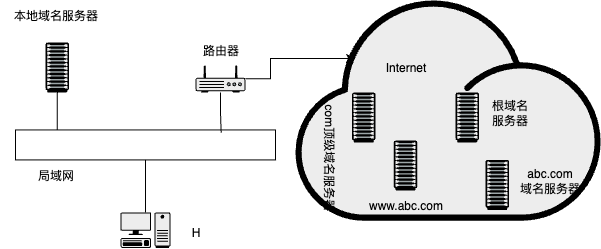
\includegraphics[scale=0.6]{计网图1.png}
    \end{figure}
    A.10ms,\ 40ms\qquad B.10ms,\ 50ms\qquad C.20ms,\ 40ms\qquad D.20ms,\ 50ms

    \item 文件传输协议(FTP)的一个主要特征是() \\
    A.允许客户指明文件的类型但不允许指明文件的格式 \\
    B.不允许客户指明文件的类型但运行指明文件的格式 \\
    C.允许客户指明文件的类型与格式 \\
    D. 不允许客户指明文件的类型与格式 

    \item 匿名FTP访问通常使用()作为用户名 \\
    A.guest\qquad B.E-mail地址\qquad C.anonymous\qquad D.主机id

    \item 下列关于POP3协议的说法,()是错误的 \\
    A.由客户端而非服务器选择接收后是否将邮件保存在服务器上
    B.登录到服务器后,发送的密码是加密的 \\
    C.协议是基于ASCII码的,不能发送二进制数据 \\
    D.一个账号在服务器上只能有一个邮件接收目录 

    \item 下面的()协议中,客户机与服务器之间采用面向无连接的协议进行通信. \\
    A.FTP\qquad B.SMTP\qquad C.DNS\qquad D.http

    \item 仅需Web服务器对HTTP报文进行响应,但不需要返回请求对象时,HTTP请求报文应该使用的方法是() \\
    A.GET\qquad B.PUT\qquad C.POST\qquad D.HEAD

    \item 下列关于Cookie的说法中,错误的是() \\
    A.Cookie存储在服务器端\qquad B.Cookie是服务器产生的\\
    C.Cookie会威胁客户的隐私\qquad D.Cookie的作用是跟踪用户的访问和状态
\end{enumerate}


\newpage
\section{计算机组成原理}

\begin{enumerate}
    \item 冯$\cdot$诺依曼机的基本工作方式是(  ) \\
    A.控制流驱动方式\qquad B.多指令多数据流方式 \\
    C.微程序控制器\qquad C.数据流驱动方式 
    
    \item \bt 将高级语言源程序转换为机器级目标文件的程序是(   ) \\
    A.汇编程序\qquad B.连接程序\qquad C.编译程序\qquad D.解释程序 

    \item 在计算机中,CPU的CPI与下列(   )因素无关.\\
    A.时钟频率\qquad B.系统结构\qquad C.指令集\qquad D.计算机组织 

    \item 某计算机主频为$1GHz$,程序P运行过程中,共执行了$10000$条指令,其中,$80\%$的指令执行平均
    需要1个始终周期,$20\%$的指令执行平均需10个时钟周期.程序P的平均CPI和CPU执行时间分别是(   ) \\
    A.$2.8,28\mu s$\qquad B.$28,28\mu s$\qquad C.$2.8,28ms$\qquad D.$28,28ms$ 

    \item 若$X$为负数,则由$[X]_{\text{补}}$求$[-X]_{\text{补}}$是将(   ) \\
    A.$[X]_{\text{补}}$各值保持不变 \\
    B.$[X]_{\text{补}}$符号位变反,其他位不变 \\
    C.$[X]_{\text{补}}$除符号位外,其余位取反,末尾加一 \\
    D.$[X]_{\text{补}}$连同符号位一起变反,末尾加一 

    \item 对于相同位数(设N位,不考虑符号位)的二进制补码小数和十进制小数,二进制小数能表示的数的个数/十进制
    小说所能表示的个数为(  ) \\
    A.$(0.2)^{N}$\qquad B.$(0.2)^{N-1}$\qquad C.$(0.02)^{N}$\qquad D.$(0.02)^{N-1}$ 

    \item 设$x$为真值,$x^{*}$为其绝对值,满足$[-x^*]_{\text{补}}=[-x]_{\text{补}}$当且仅当x为(   ) \\
    A.任意数 \qquad B.正数\qquad C.负数\qquad D.以上说法均不正确

    \item ALU作为运算器的核心部件,其属于(   ) \\
    A.时序逻辑电路\qquad B.组合逻辑电路\qquad C.控制器\qquad D.寄存器 

    \item \bl 加法器中每位的进位信号由(   )组成\\
    A.$X_i\oplus Y_i$\qquad B.$X_iY_i$ \qquad C.$X_iY_iC_i$\qquad D.$X_i+Y_i+C_i$ 

    \item 一个8位寄存器内的数值为\underline{1100\ 1010}进位标志位寄存器C为0,若将此8位寄存器循环左移
    1位后,则该寄存器和标志寄存器的值分别为(   ) \\
    A.1001\ 0100, 1\qquad B.1001\ 0101, 0\qquad C.1001\ 0101, 1\qquad D.1001\ 0100, 0

    \item 设机器数字长8位(含一位符号位),若机器数为$BAH$为原码,算术左移1和算术右移1位分别得(   ) \\
    A.$F4H,EDH$\qquad B.$B4H,6DH$\qquad C.$74H,DDH$\qquad D.$B5H,EDH$ 

    \item 关于模4补码,下列说法中正确的是(   ) \\
    A.模4补码和模2补码不同,它不容易检查乘除运算中的溢出问题 \\
    B.每个模4补码存储时只需要存储一位符号位 \\
    C.存储每个模4补码需要存储两个符号位\\ 
    D.模4补码,在算术与逻辑部件中为一个符号位 

    \item 在原码一位乘法中,(   ) \\
    A.符号位参与运算 \\
    B.符号位不参与运算 \\
    C.符号位参与运算,并根据运算结果改变结果中的符号位 \\
    D.符号位不参与运算,并根据运算结果改变结果中的符号位

    \item \bl 某计算机字长为8位,CPU中有一个8位加法器.已知无符号数$x=69,y=38$,如果在该加法器中计算x-y,则加法
    器的两个输入端入端信息和低位进位信息分别是() \\
    A.0100\ 0101,0010\ 0110, 0 \qquad B.0100\ 0101,1101\ 1001, 1 \\
    C.0100\ 0101,1101\ 1010, 0 \qquad D.0100\ 0101,1101\ 1010, 1

    \item \bt 某计算机存储器按字节编制,采用小端方式存放数据.假定编译器规定int型和short型长度分别为32位和16位
    并且数据按边界对齐存储.某C语言程序段如下
\begin{lstlisting}[language=C]
    struct {
        int a;
        char b;
        short c;
    }record;
    record.a = 273;
\end{lstlisting}
    若record变量的首地址为0xC008地址0xC008中的内容及record.c的地址分别是()
    A.0x00, 0xC00D\qquad B.0x00,0xC00E\qquad C.0x11,0xC00D \qquad D.0x11,0xC00E 

    \item \bt 有如下C语言序段:
\begin{lstlisting}[language=C]
    short si = -32767;
    unsigned short usi = si;
\end{lstlisting}
    这执行上述两条语句后,usi的值是\_\_\_\_ 

    \item 某计算机字长为32位,按字节编址,采用小端方式存放数据,假定有一个$double$型变量,其机器数表示
    为1122\ 3344\ 5566\ 7788H,存放在以0000\ 8040H开始的连续存储单元中,则存储单元0000\ 8046H中存储的是(   )\\
    A.22H\qquad B.33H\qquad C.77H\qquad D.66H 

    \item 在规格化浮点运算中,若浮点数$2^5\times1.10101$,其中尾数为补码表示,则该数(   ) \\
    A.不需要规格化\qquad B.需要右移规格化 \\
    C.需将尾数左移一位规格化\qquad D.需将尾数左移二位规格化 

    \item 某浮点机,采用规格化浮点数表示,阶码用移码表示(最高位表示符号位),尾数用原码表示,下列(   )表示不是规格化浮点数 \\
    A.1111111, 1.10000...000 \qquad B.0011111, 1.0111...01 \\
    B.1000001, 0.11111...111 \qquad D.0111111, 0.100000000 

    \item 下列关于对阶操作说法正确的是(   ) \\
    A. 在浮点数加减运算对阶操作中,若阶码减少,则尾数左移 \\
    B. 在浮点数加减运算对阶操作中,若阶码增大,则尾数右移;若阶码减少,则尾数左移 \\
    C. 在浮点数加减运算对阶操作中,若阶码增大,则尾数右移 \\
    D. 以上说法都不对 

    \item 在$IEEE\ 754$标准中,它所能表示的最小规格化负数为(    )

    \item 采用规格化的浮点数最主要是为了(   ) \\
    A.增加数据的表示范围\qquad B.方便浮点运算\\
    C.防止运算时数据溢出\qquad D.增加数据的表示精度 

    \item 设浮点数共12位,其中阶码以4位补码表示(1位符号),尾数用8位补码表示(1为符号).则该规格化浮点数
    所能表示的最大正数为(    ) 

    \item 若浮点数的尾数用补码表示,则下列(   )中的尾数是规格化形式 \\
    A.1.11000\qquad B.0.01110\qquad C.0.01010\qquad D.1.00010 

    \item 设浮点数的基数为4,尾数用原码表示,则以下(   )是规格化的数 \\
    A.1.001101\qquad B.0.001101\qquad C.1.011011\qquad D.0.000010 

    \item 下列关于舍入的说法,正确的是(多选)(   )
    \begin{enumerate}
        \item [(1)] 不仅仅只有浮点数需要舍入,定点数在运算时也可能舍入 
        \item [(2)] 在浮点数舍入中,只有左规格化时可能舍入
        \item [(3)] 在浮点数舍入中,只有右规格化时可能舍入
        \item [(4)] 在浮点数舍入中,左,右规格化时都可能舍入
        \item [(5)] 舍入不一定能产生误差
    \end{enumerate}

    \item \bt 假定变量$i,f,d$的数据类型分别是$int,float,double$(int用补码表示,其余用IEEE\ 754浮点
    数格式),已知$i=785,f=1.5678E3,d=1.5E100$,若在$32$位机器中执行下列关系表达式,则结果为真的是(多选)(   )
    \begin{enumerate}
        \item [(1)] $i==(int)(float)i$ 
        \item [(2)] $f==(float)(int)f$ 
        \item [(3)] $f==(float)(double)f$
        \item [(4)] $(d+f)-d==f$
    \end{enumerate}

    \item \bt $flota$类型数据通常用IEEE\ 754单精度格式表示,若编译器将$float$型变量$x$分配在一个
    32位浮点寄存器$FR1$中,且$x=-8.25$则$FR1$中的内容是\_\_\_\_ 

    \item \bt 下列关于浮点数加减运算中,正确的是(多选)(    )
    \begin{enumerate}
        \item [(1)] 对阶操作不会引起阶码上溢或下溢 
        \item [(2)] 右规和尾数舍入都可以引起阶码上溢 
        \item [(3)] 左规时可能引起阶码下溢 
        \item [(4)] 尾数溢出时结果不一定溢出 
    \end{enumerate}

    \item \bt 假定用若干$2K\times 4$的芯片组成一个$8K\times 8$的存储器,则地址081FH所在芯片的
    最小地址是(    ) \\
    A.0000H\qquad B.0600H\qquad C.0700H\qquad D.0800H 

    \item \bt 某计算机存储器按字节编址,主存地址空间大小为$64MB$,现用$4M\times 8$位的RAM芯片组成
    32MB的主存储器,则存储器地址寄存器$MAR$的位数至少是\_\_\_\_ 

    \item \bt 某磁盘的转速为$10000$转/分,平均寻道时间是$6ms$,磁盘传输速率是$20MB/s$磁盘控制器延迟
    为$0.2ms$,读取一个$4KB$的扇区所需要的平均时间约为(   ) \\
    A.$9ms$\qquad B.$9.4ms$\qquad C.$12ms$\qquad D.$12.4ms$

    \item \bt 假设主存地址为32位,按字节编址,主存和Cache之间采用直接映射方式,主存块大小为4个字,每个字32位,
    采用回写方式,则能存放4K字数据的Cache总容量的位数至少是(   ) \\
    A.146K\qquad B.147K\qquad C.148K\qquad D.158K 

    \item \bl 一个计算机系统采用32位单字长指令,地址码12位,若定义了250条二地址指令,则还可以有(   )单地址指令. \\
    A.4K\qquad B.8K\qquad C.16K\qquad D.24K 

    \item \bt 下列选项中,属于指令集体系结构(ISA)规定的内容是(多选)(    )
    \begin{enumerate}
        \item [(1)] 指令字格式和指令类型 
        \item [(2)] CPU的时钟周期 
        \item [(3)] 同样寄存器个数和位数 
        \item [(4)] 加法器的进位方式
    \end{enumerate}

    \item \bt 设计某指令系统时,假设采用16位定长指令格式,操作码使用拓展编码方式,地址码为6位,包括零
    地址,一地址和二地址三种指令.若二地址指令有12条,一地址指令有254条,则零地址指令的条数最多为(   )\\
    A.0\qquad B.2\qquad C.64\qquad D.128

    \item 指令系统中采用不同寻址方式的目的是(   )\\
    A.提供拓展操作码的可能性并降低译码难度 \\
    B.可缩短指令字长,托大寻址空间,提高编程的灵活性 \\
    C.实现程序控制 \\
    D.三者都正确 

    \item 简化地址结构的基本方法是尽量采用(   ) \\
    A.寄存器寻址\qquad B.隐含寻址\qquad C.直接寻址\qquad D.间接寻址 

    \item 在多道程序设计中,最重要的寻址方式是(   ) \\
    A.相对寻址\qquad B.间接寻址\qquad C.立即寻址\qquad D.按内容寻址
    
    \item 设相对寻址的转移指令占3B,第一字节为操作码,第二、三字节为相对位移量(补码 表示),
    而且数据在存储器中采用以低字节为字地址的存放方式。每当CPU从存储器取 出一字节时,
    即自动完成(PC)+1$\rightarrow$PC。若PC的当前值为240 (十进制),要求转移到 290 (十进制),
    则转移指令的第二、三字节的机器代码是();若PC的当前值为240 (十进制),要求转移到200 (十进制),
    则转移指令的第二、三字节的机器代码是()。 \\
    A.2FH,FFH \qquad B.D5H,00H\qquad C.D5H,FFH\qquad D.2FH,00H

    \item 】某计算机有16个通用寄存器,采用32位定长指令字,操作码字段(含寻址方式位)为8位,Store指令的源操作数和目的操作数分别采用寄存器直接寻址和 基址寻址方式。
    若基址寄存器可使用任意一个通用寄存器,且偏移量用补码表示,则Store 指令中偏移量的取值范围是(   ) \\
    A.$-32768\sim +32767$\qquad B.$-32767\sim +32768$ \\
    B.$=65536\sim +65535$\qquad D.$-65535\sim +65536$ 

    \item 按字节编址的计算机中,某double型数组A的首地址为2000H,使用变址寻址和循环结构访问数组A,
    保存数组下标的变址寄存器的初值为0,每次循环取一个数组元素,其偏移地址为变址值乘以
    sizeof(double),取完后变址寄存器的内容自动加1。若某次循环所取元素的地址为2100H,
    则进入该次循环时变址寄存器的内容是(   ) \\
    A.25\qquad B.32\qquad C.64\qquad D.100 

\end{enumerate}

\newpage
\section{操作系统}

\begin{enumerate}
    \item 系统调用是由操作系统提供给用户的,它() \\
    A.直接通过键盘交互方式使用\qquad B.只能通过用户程序间接使用 \\
    C.是命令接口中的命令\qquad D.与系统的命令一样
    
    \item 操作系统与用户通信接口通常不包括() \\
    A.shell\qquad B.命令解释器\qquad C.广义指令\qquad D.缓存管理指令 

    \item 下列关于多道程序系统的叙述中,不正确的是() \\
    A.支持程序的并发执行\qquad B.不必支持虚拟存储管理 \\
    C.需要实现对共享资源的管理\qquad D.进程数越多CPU利用率也越多 

    \item 分时系统的一个重要指标是系统的响应时间,对操作系统的()因素改进有利于改善操作系统的响应时间. \\
    A.加大时间片\qquad B.采用静态页式管理 \\
    C.优先级+非抢占式调度算法\qquad D.代码可重入 

    \item 计算机区分内核态和用户态指令后,从核心态到用户态的转变用操作系统执行后完成,而用户态转换到核心态则有()完成 \\
    A. 硬件\qquad B.核心态程序\qquad C.用户程序\qquad D.中断处理程序

    \item "访管"指令()使用 \\
    A. 仅在用户态\qquad B.仅在内核态\qquad C.在规定时间内\qquad D.在调度时间内

    \item 在操作系统中,只能在核心态下执行的指令是() \\
    A. 读时钟\qquad B.取数\qquad C.广义指令\qquad D.寄存器清零

    \item \bt\bl 中断处理和子程序调用都需要压栈以保护现场,中断处理一定会保存而子程序调用不一定需要保存的内容是() \\
    A. 程序计数器\qquad B.程序状态字寄存器\qquad C.通用寄存器组\qquad D.通用地址寄存器

    \item \bt 定时器产生时钟中断后,由时钟中断服务程序更新的内容是()
    \begin{enumerate}
        \item [I] 内核中时间变量的值
        \item [II] 当前进程占用的CPU时间
        \item [III] 当前进程在时间片中的剩余执行时间
    \end{enumerate}
    A.仅I,II\qquad B.仅II,III\qquad C.仅I,III\qquad D.I,II,III

    \item \bt\bl 下列与中断相关的操作中,由操作系统完成的是(多选)()  
    \begin{enumerate}
        \item [I] 保存中断点
        \item [II] 提供中断服务
        \item [III] 初始化中断向量表
        \item [IV] 保存中断屏蔽字
    \end{enumerate}

    \item \bl 计算机的启动过程是(排序)() 
    \begin{enumerate}
        \item [1] CPU加点, CS:IP指向FFFF0H
        \item [2] 进行操作系统引导
        \item [3] 执行JMP指令跳转到BIOS
        \item [4] 登记BIOS中断例程入口地址
        \item [5] 硬件自检
    \end{enumerate}

    \item 在单处理机系统中,若同时存在10个进程,则处于就绪队列的进程最多有() \\
    A. 10个\qquad B.9个\qquad C.8个\qquad D.7个 

    \item 进程在处理器上执行时,() \\
    A. 进程之间是无关的,且具有封闭特性 \\
    B. 进程之间都有交互性,相互依赖,相互制约,具有并发性 \\
    C. 具有并发性,即同时执行的特性 \\
    D. 进程之间可能是无关的,但也可能是具有交互性的

    \item 在多对一的线程模型中,当一个多线程中的某线程被阻塞后() \\
    A. 该进程的其他线程仍然能够运行 \qquad B. 整个进程将被阻塞 \\
    C. 该阻塞进程将被撤销\qquad D. 该阻塞线程将永远不能再执行 

    \item 系统动态DLL库中的系统线程,被不同的进程所调用,它们是()的线程 \\
    A. 不同\qquad B.相同\qquad C.可能不同,可能相同\qquad D.不能被调用

    \item 下列不是多线程系统特长的是() \\
    A. 利用线程可以并发地执行矩阵乘法计算 \\
    B. Web服务器利用线程响应HTTP请求 \\
    C.键盘驱动程序为每个正在运行的程序配备一个线程,用以响应用户的输入 \\
    D. 基于GUI的调试程序用不同的线程分别处理用户输入,计算和跟踪等操作

    \item 下列选中,导致创建新进程的操作是(多选)() \\
    I.用户登录成功\qquad II.设备分配\qquad III,启动用户执行

    \item 可能导致进程被唤醒的事件是(多选)() \\
    I. I/O结束\qquad II.某进程退出临界区\qquad III.当前进程的时间片用完 

    \item 下列关于父进程与子进程的说法中错误的是() \\
    A.父进程和子进程可以并发执行 \\
    B.父进程和子进程共享虚拟地址空间 \\
    C.父进程和子进程有不同进程控制块 \\
    D.父进程和子进程共享临界资源

    \item 一个作业8:00到达系统,估计运行时间为1h,若10:00开始执行作业,其响应比为()

    \item 在进程调度算法中对短进程不利的是() \\
    A. 短进程优先调度\qquad B.先来先服务调度 \\
    C.高响应比优先调度算法\qquad D.多级反馈优先队列

    \item 不需要信号量就能实现的功能是() \\
    A.进程同步\qquad B.进程互斥\qquad C.进程的前驱关系\qquad D.进程的并发执行

    \item 若一个信号量的初始值为3,经过多次PV操作后当前值为-1,这表示进入临界区的进程数是() \\
    A. 1\qquad B.2\qquad C.3\qquad D.4

    \item 以下()属于临界资源 \\
    A. 打印机\qquad B.公用队列\qquad C.私有数据\qquad D.可重入的程序代码 

    \item 一个进程因在互斥信号量mutex上执行V操作而导致唤醒另一个进程的时,执行V操作后mutex的值为() \\
    A.大于0\qquad B.小于0\qquad C.大于等于0\qquad D.小于等于0 

    \item 进程P1和进程P2均包含并发执行的线程,部分伪代码如下,下列选项中,需要互斥执行的操作是() 
    \begin{center}
        \begin{minipage}[t]{0.45\textwidth}
\begin{lstlisting}[language=C, numbers=left]
// 进程P1                    
int x = 0;                   
Thread1() {                  
    int a;
    a = 1;
    x += 1;
}
Thread2() {
    int a;
    a = 2;
    x += 2;
}
\end{lstlisting}
        \end{minipage}
        \hfill
        \begin{minipage}[t]{0.45\textwidth}
\begin{lstlisting}[language=C]
// 进程P2                    
int x = 0;                   
Thread3() {                  
    int a;
    a = x;
    x += 3;
}
Thread4() {
    int a;
    b = x;
    x += 4;
}
\end{lstlisting}
        \end{minipage}
    \end{center}

    A.a=1与a=2\qquad B. a=x与b=x\qquad C.x +=1 与 x+=2\qquad D.x+=1与x+=3
    \item 下面是一个并发进程的程序代码,正确的是() 
    \begin{center}
        \begin{minipage}[t]{0.45\textwidth}
            \begin{lstlisting}[language=C, numbers=left]
Semaphore x1=x2=y=1;
int c1=c2=0;
P1() {
    while(1) {
        P(x1);
        if(++c1 == c) P(y);
        V(x1);
        computer(A);
        P(x1);
        if(--c1 == 0) V(y);
        V(x1);
    }
}
                \end{lstlisting}
            \end{minipage}
            \hfil
            \begin{minipage}[t]{0.45\textwidth}
                \begin{lstlisting}
Semaphore x1=x2=y=1;
int c1=c2=0;
P2() {
    while(1) {
        P(x2);
        if(++c2 == 1) P(y);
        V(x2);
        computer(B);
        P(x2);
        if(--c2 == 0) V(y);
        V(x2);
    }
}
            \end{lstlisting}
        \end{minipage}
    \end{center}
A.进程不会死锁,也不会饥饿 \qquad B.进程不会死锁,但会饥饿 \\
C.进程会死锁,但是不会饥饿\qquad D.进程会死锁,也会饥饿 

    \item 有两个并发进程,对于如这段程序的执行,正确的是() 
\begin{center}
    \begin{minipage}[t]{0.45\textwidth}
        \begin{lstlisting}[numbers=left]
int x, y, z, t, u;
P1() {
    while(1) {
        x = 1;
        y = 0;
        if (x >= 1) y = y + 1;
        z = y;
    }
}
    \end{lstlisting}
\end{minipage}
\hfil
\begin{minipage}[t]{0.45\textwidth}
    \begin{lstlisting}
int x, y, z, t, u;
P2() {
    while(1) {
        x = 0;
        t = 0;
        if (x <= 1) t = t + 1;
        u = t;
    }
}
            \end{lstlisting}
        \end{minipage}
    \end{center}
    A.程序能够正常运行,结果唯一\qquad B.程序不能正常运行,可能出现两种结果\\
    C.程序不能正常运行,结果不确定\qquad D.程序不能正确运行,可能会死锁


    \item 若系统S1采用死锁避免方法,S2采用死锁检查方法,下列叙述中,正确的是(多选)() \\
    I. S1会限制用户申请资源的顺序,而S2不会 \\
    II. S1需要进程运行所需要的资源信息,而S2不需要 \\
    III. S1不会给可能导致死锁的进程分配资源,但S2会

    \item 下列存储管理方案中,()方式可以采用静态重定位 \\
    A.固定分区\qquad B.可变分区\qquad C.页式\qquad D.段式

    \item 下列不会产生内部碎片的存储管理是() \\
    A.分页式\qquad B.分段式\qquad C.段页式\qquad D.固定分区

    \item 采用分页和分段管理后,提供给用户的物理地址空间() \\
    A.分页支持更大的物理地址空间\qquad B.分段支持更大的物理地址空间 \\
    C.不能确定\qquad D.一样大

    \item 可重入程序是通过()方法来改善系统性能的. \\
    A.改变时间片长度\qquad B.改变用户数\qquad C.提供对换速度\qquad D.减少对换数量 

    \item 对主存储器的访问() \\
    A.以块(页)为单位 \qquad B.以字节或字位单位 \\
    C.随存储器的管理方案有所不同\qquad D.以用户的逻辑记录为单位

    \item 操作系统采用分页存储管理,要求() \\
    A.每个进程拥有一张页表,且进程的页表驻留在内存中 \\
    B.每个进程拥有一张页表,仅运行的进程的页表驻留在内存中\\
    C.所有进程共享一张页表,以节约有限的内存空间,但页表必须驻留在内存中 \\
    D.每个进程共享一张页表,只有页表中当前使用的页表必须驻留以最大限度节约有限的内存空间

    \item 在下列动态分区分配算法中,最容易产生内部碎片的是()  \\
    A.首次适应算法\qquad B.最坏适应算法\qquad C.最佳适应算法\qquad D.循环首次适应算法

    \item 请求分页存储管理中,若把页面尺寸增大一倍且可容纳的最大页数不变,则在程序顺序执行时缺页中断次数
    将会() \\
    A.增加\qquad B.减少\qquad C.不变\qquad D.无法确定

    \item 考虑页面置换算法,系统有m个物理块供调度,初始时全空,页面引用串长度为p,包含n个不同的页号,无论用啥算法
    缺页次数不会少于()

    \item 设主存容量为1MB,外存容量为400MB,计算机系统的地址寄存器有32位,那么虚拟存储器的最大容量是() 

    \item 导致LRU算法实现起来消耗特高的原因是() \\
    A.需要特殊硬件支持\qquad B.需要特殊的中断处理程序 \\
    C.需要在页表中标明特殊的页类型\qquad D.需要对所有页进行排序

\end{enumerate}

\ifx\allfiles\undefined
\end{document}
\fi